\documentclass[a4paper,12pt,fleqn]{article}%fleqn pour aligner les equations à gauche
\usepackage{../../Styles/Cours}


\newcommand{\chnum}{Chapitre 1}
\newcommand{\chtitle}{Détermination du volume molaire d'un gaz}
\newcommand{\dtype}{TP 2}

\begin{document}
	\maketitle
L'état gazeux est l'état physique le moins accessible vis-à-vis des mesures physiques. L'objectif de cette activité est d'accéder au volume molaire de gaz lors de deux réactions chimiques et de déterminer le volume molaire des gaz produits.

\begin{figure}[h!]
	\caption{Dispositif expérimental}
	\label{doc1}
	\centering 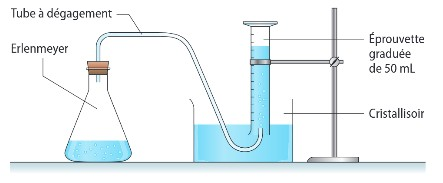
\includegraphics[width =.6\linewidth]{Ressources/1SPE_C1_AE2_Fig1.png}
\end{figure}
	
\begin{figure}[h!]
	\caption{Protocole expérimental}
	\label{doc2}
	\begin{itemize**}
		\item Remplir à moitié un cristallisoir et complètement une éprouvette graduée d'eau du robinet.
		\item Boucher l'éprouvette et la renverser sur le cristallisoir, puis la déboucher et la fixer par une pince, enfin placer en-dessous un tube à dégagement.
		\item Dans un erlenmeyer, introduire les espèces chimiques nécessaires à la production du gaz, puis placer rapidement le tube à dégagement sur l'erlenmeyer.
		\item Attendre la fin de la réaction et noter le volume de gaz recueilli.
	\end{itemize**}
	
	\caption{Réactions à mettre en place}
	\label{doc3}
	\begin{tabular}{|m{.48\linewidth}|m{.48\linewidth}|}
		\hline
		Production de dioxyde de carbone & Production de dihydrogène\\
		\hline
		\begin{itemize**}
			\item Introduire dans l'erlenmeyer dans \SI{10}{mL} d'eau distillée, prélevés à l'éprouvette graduée
			\item Ajouter \SI{1.0}{mL} de solution d'acide chlorhydrique, prélevé à la pipette jaugée, puis une spatule d'hydrogénocarbonate de sodium.
			\item Boucher rapidement.
		\end{itemize**} & \begin{itemize**}
		\item Introduire dans l'erlenmeyer \SI{10}{mL} de la solution d'acide chlorhydrique, prélevés à l'éprouvette graduée.
		\item Ajouter \SI{2,1}{cm} de ruban de magnésium et boucher rapidement.
		\end{itemize**}\\
		\hline
	\end{tabular}
\end{figure}

\begin{figure}[h!]
	\caption{Données :}
	\label{doc4}
	\begin{itemize}
		\item Masse linéique du ruban de magnésium : $\mu = \SI{1,147}{\gram\per\meter}$
		\item Concentration molaire de la solution d'acide chlorhydrique : $C=\SI{1,0}{\mole\per\liter}$
		\item Équation de la réaction 1 : \ce{NaHCO3(s) + H3O+(aq) -> CO2(g) + Na+(aq) + 2H2O(l)}
		\item Équation de la réaction 1 : \ce{Mg(s) + 2H3O+(aq) -> Mg^2+(aq) + H2(g) + 2H2O(l) }
	\end{itemize}
\end{figure}

\begin{figure}[h!]
	\caption*{Questions :}
	\begin{enumerate}
		\item Déterminer la quantité initiale d'ions oxonium, \ce{H3O+}, mise en jeu dans la réaction 1.
		\item Déterminer la quantité de matière initiale de magnésium dans la réaction 2.
		3. Vérifier que chaque réaction produise \SI{1,0E-3}{\mole} de gaz.
	\end{enumerate}
	\textit{Réaliser \emph{une des deux expériences} en suivant les conseils du professeur.}
	
	\begin{enumerate}[resume]
		\item Déterminer le volume occupé par une mole de gaz pour chaque expérience.
		\item La loi d'\textit{Avogadro-Ampère} dit que le volume des gaz est indépendant de la nature des gaz, pour une pression et une température données. Donner une estimation du volume molaire des gaz en \unit{\liter\per\mole}.
		\item Proposer une explication au fait que la loi d'Avogadro-Ampère ne soit qu’approximativement respectée par l'expérience. Proposer des moyens pour améliorer la qualité des mesures effectuées. 
	\end{enumerate}
\end{figure}

	
\end{document}